% Judul dokumen
\title{Buku Tugas Akhir ITS}
\author{Musk, Elon Reeve}

% Pengaturan ukuran teks dan bentuk halaman dua sisi
\documentclass[12pt,twoside]{report}

% Pengaturan ukuran halaman dan margin
\usepackage[a4paper,top=30mm,left=30mm,right=20mm,bottom=25mm]{geometry}

% Pengaturan ukuran spasi
\usepackage[singlespacing]{setspace}

% Pengaturan format bahasa
\usepackage[indonesian]{babel}

% Pengaturan detail pada file PDF
\usepackage[pdfauthor={\@author},bookmarksnumbered,pdfborder={0 0 0}]{hyperref}

% Pengaturan jenis karakter
\usepackage[utf8]{inputenc}

% Pengaturan pewarnaan
\usepackage[table,xcdraw]{xcolor}

% Pengaturan kutipan artikel
\usepackage[numbers]{natbib}

% Package lainnya
\usepackage{changepage}
\usepackage{enumitem}
\usepackage{eso-pic}
\usepackage{etoolbox}
\usepackage{graphicx}
\usepackage{lipsum}
\usepackage{lmodern}
\usepackage{longtable}
\usepackage{tabularx}
\usepackage{wrapfig}

% Definisi untuk "Hati ini sengaja dikosongkan"
\patchcmd{\cleardoublepage}{\hbox{}}{
  \thispagestyle{empty}
  \vspace*{\fill}
  \begin{center}\textit{[Halaman ini sengaja dikosongkan]}\end{center}
  \vfill}{}{}

% Pengaturan penomoran halaman
\usepackage{fancyhdr}
\fancyhf{}
\renewcommand{\headrulewidth}{0pt}
\pagestyle{fancy}
\fancyfoot[RE,RO]{\thepage}
\patchcmd{\chapter}{plain}{fancy}{}{}
\patchcmd{\chapter}{empty}{plain}{}{}

% Pengaturan format judul bab
\usepackage{titlesec}
\titleformat{\chapter}[display]{\bfseries\Large}{BAB \centering\Roman{chapter}}{0ex}{\vspace{0ex}\centering}
\titleformat{\section}{\bfseries\large}{\MakeUppercase{\thesection}}{1ex}{\vspace{1ex}}
\titleformat{\subsection}{\bfseries\large}{\MakeUppercase{\thesubsection}}{1ex}{}
\titleformat{\subsubsection}{\bfseries\large}{\MakeUppercase{\thesubsubsection}}{1ex}{}
\titlespacing{\chapter}{0ex}{0ex}{4ex}
\titlespacing{\section}{0ex}{1ex}{0ex}
\titlespacing{\subsection}{0ex}{0.5ex}{0ex}
\titlespacing{\subsubsection}{0ex}{0.5ex}{0ex}

% Pengaturan format potongan kode
\usepackage{listings}
\definecolor{comment}{RGB}{0,128,0}
\definecolor{string}{RGB}{255,0,0}
\definecolor{keyword}{RGB}{0,0,255}
\lstdefinestyle{codestyle}{
  commentstyle=\color{comment},
  stringstyle=\color{string},
  keywordstyle=\color{keyword},
  basicstyle=\footnotesize\ttfamily,
  numbers=left,
  numberstyle=\tiny,
  numbersep=5pt,
  frame=lines,
  breaklines=true,
  prebreak=\raisebox{0ex}[0ex][0ex]{\ensuremath{\hookleftarrow}},
  showstringspaces=false,
  upquote=true,
  tabsize=2,
}
\lstset{style=codestyle}

% Isi keseluruhan dokumen
\begin{document}

  % Sampul luar Bahasa Indonesia
  \newcommand\covercontents{sampul/konten-id.tex}
  \AddToShipoutPictureBG*{
  \AtPageLowerLeft{
    % Ubah nilai berikut jika posisi horizontal background tidak sesuai
    \hspace{-3.5mm}

    % Ubah nilai berikut jika posisi vertikal background tidak sesuai
    \raisebox{0mm}{
      
\includegraphics[width=\paperwidth,height=\paperheight]{sampul/gambar/sampul-luar2.png}
    }
  }
}

% Menyembunyikan nomor halaman
\thispagestyle{empty}

% Pengaturan margin untuk menyesuaikan konten sampul
\newgeometry{
  top=55mm,
  left=30mm,
  right=20mm,
  bottom=25mm
}

\begin{flushleft}
  % Pemilihan font sans serif
  \sffamily

  % Pemilihan warna font putih
  \color{white}

  % Pemilihan font bold
  % \fontseries{bx}
  \selectfont

  \input{\covercontents}

\end{flushleft}

\restoregeometry


  % Atur ulang penomoran halaman
  \setcounter{page}{1}

  % Sampul dalam Bahasa Indonesia
  \renewcommand\covercontents{sampul/konten-id.tex}
  \AddToShipoutPictureBG*{
  \AtPageLowerLeft{
    % Ubah nilai berikut jika posisi horizontal background tidak sesuai
    \hspace{-3.5mm}

    % Ubah nilai berikut jika posisi vertikal background tidak sesuai
    \raisebox{0mm}{
      
\includegraphics[width=\paperwidth,height=\paperheight]{sampul/gambar/sampul-dalam2.png}
    }
  }
}

% Menyembunyikan nomor halaman
\thispagestyle{empty}

% Pengaturan margin untuk menyesuaikan konten sampul
\newgeometry{
  top=65mm,
  left=30mm,
  right=20mm,
  bottom=25mm
}

\begin{flushleft}

  % Pemilihan font sans serif
  \sffamily

  % Pemilihan font bold
  % \fontseries{bx}
  \selectfont

  \input{\covercontents}

\end{flushleft}

\restoregeometry

  \clearpage
  \cleardoublepage

  % Sampul dalam Bahasa Inggris
  \renewcommand\covercontents{sampul/konten-en.tex}
  \AddToShipoutPictureBG*{
  \AtPageLowerLeft{
    % Ubah nilai berikut jika posisi horizontal background tidak sesuai
    \hspace{-3.5mm}

    % Ubah nilai berikut jika posisi vertikal background tidak sesuai
    \raisebox{0mm}{
      
\includegraphics[width=\paperwidth,height=\paperheight]{sampul/gambar/sampul-dalam2.png}
    }
  }
}

% Menyembunyikan nomor halaman
\thispagestyle{empty}

% Pengaturan margin untuk menyesuaikan konten sampul
\newgeometry{
  top=65mm,
  left=30mm,
  right=20mm,
  bottom=25mm
}

\begin{flushleft}

  % Pemilihan font sans serif
  \sffamily

  % Pemilihan font bold
  % \fontseries{bx}
  \selectfont

  \input{\covercontents}

\end{flushleft}

\restoregeometry

  \cleardoublepage

  % Pengaturan ukuran indentasi paragraf
  \setlength{\parindent}{2em}

  % Pengaturan ukuran spasi paragraf
  \setlength{\parskip}{1ex}

  % Lembar pengesahan
  \begin{center}
	\large
  \textbf{LEMBAR PENGESAHAN}
\end{center}

% Menyembunyikan nomor halaman
\thispagestyle{empty}

\begin{center}
  % Ubah kalimat berikut dengan judul tugas akhir
  \textbf{\emph{ETHER WALLET} MENGGUNAKAN \emph{ETHEREUM} BERBASIS \emph{PROOF OF STAKE}}
\end{center}

\begingroup
  % Pemilihan font ukuran small
  \small
  
  \vspace{3ex}

  \begin{center}
    \textbf{PROPOSAL TUGAS AKHIR}
    \\Diajukan untuk memenuhi salah satu syarat
    \\memperoleh gelar Sarjana pada
    \\Program Studi S-1 Teknik Komputer
    \\Departemen Teknik Komputer
    \\Fakultas Teknologi Elektro dan Informatika Cerdas
    \\Institut Teknologi Sepuluh Nopember
  \end{center}

  \vspace{3ex}

  \begin{center}
    % Ubah kalimat berikut dengan nama dan NRP mahasiswa
    Oleh: Dimas Nazli Bahaduri 
    \\NRP. 0721 18 4000 0060
  \end{center}

  \vspace{3ex}

  % \begin{center}
  % Ubah kalimat-kalimat berikut dengan tanggal ujian dan periode wisuda
  %   Tanggal Ujian : 1 Juni 2021\\
  %   Periode Wisuda : September 2021
  % \end{center}

  \begin{center}
    Disetujui oleh Tim Penguji Tugas Akhir:
  \end{center}

  \vspace{4ex}

  \begingroup
    % Menghilangkan padding
    \setlength{\tabcolsep}{0pt}

    \noindent
    \begin{tabularx}{\textwidth}{X l}
      % Ubah kalimat-kalimat berikut dengan nama dosen pembimbing pertama
      1. Mochamad Hariadi, S.T., M.Sc., Ph.D.          & Pembimbing 1 \\
      % NIP: 18560710 194301 1 001        & ................................... \\
      &  NIP 196912091997031002\\
      &  \\
      % Ubah kalimat-kalimat berikut dengan nama dosen pembimbing kedua
      2. Dr. Supeno Mardi Susiki Nugroho, S.T., M.T.     & Pembimbing 2 \\
      &  NIP 197003131995121001\\
      &  \\
      % Ubah kalimat-kalimat berikut dengan nama dosen penguji pertama
      3. Dr. Galileo Galilei, S.T., M.Sc.  & Penguji I \\
      &  \\
      &  \\
      % Ubah kalimat-kalimat berikut dengan nama dosen penguji kedua
      4. Friedrich Nietzsche, S.T., M.Sc.  & Penguji II \\
      &  \\
      &  \\
      % Ubah kalimat-kalimat berikut dengan nama dosen penguji ketiga
      5. Alan Turing, ST., MT.             & Penguji III \\
      &  \\
      &  \\
    \end{tabularx}
  \endgroup

  \vspace{12ex}

  % \begin{center}
  %   % Ubah kalimat berikut dengan jabatan kepala departemen
  %   Mengetahui, \\
  %   Kepala Departemen Teknik Dirgantara FTD - ITS \\

  %   \vspace{8ex}

  %   % Ubah kalimat-kalimat berikut dengan nama dan NIP kepala departemen
  %   \underline{Dr. Leonardo Da Vinci, S.T., M.T.} \\
  %   NIP. 14520415 151905 1 001
  % \end{center}

  \begin{center}
    \textbf{SURABAYA\\Mei, 2022}
  \end{center}
\endgroup

  \cleardoublepage

  % Pernyataan keaslian
  \begin{center}
  \large
  \textbf{PERNYATAAN ORISINALITAS}
\end{center}

% Menyembunyikan nomor halaman
\thispagestyle{empty}

\vspace{2ex}

% Ubah paragraf-paragraf berikut sesuai dengan yang ingin diisi pada pernyataan keaslian

\noindent Yang bertanda tangan dibawah ini:

\noindent\begin{tabularx}{\textwidth}{X X l}
  & \\
  Nama Mahasiswa / NRP &: Dimas Nazli Bahaduri / 07211840000060 \\
  Departemen &: Departemen Teknik Komputer\\
  Dosen Pembimbing &: Mochamad Hariadi, ST., M.Sc., Ph.D. \\
  & Dr. Supeno Mardi Susiki Nugroho, ST., M.T. \\
\end{tabularx}

Dengan ini menyatakan bahwa Tugas Akhir dengan judul "\emph{Ether Wallet} Menggunakan \emph{Ethereum} Berbasis \emph{Proof of Stake}" adalah hasil karya sendiri, berfsifat orisinal, dan ditulis dengan mengikuti kaidah penulisan ilmiah.

Bilamana di kemudian hari ditemukan ketidaksesuaian dengan pernyataan ini, maka saya bersedia menerima sanksi sesuai dengan ketentuan yang berlaku di Institut Teknologi Sepuluh Nopember.

\vspace{8ex}

\noindent\begin{tabularx}{\textwidth}{X l}
  % Ubah kalimat berikut sesuai dengan tempat, bulan, dan tahun penulisan
  & Surabaya,  2022\\
  & \\
  Mengetahui & \\
  Dosen Pembimbing & Mahasiswa\\
  & \\
  & \\
  & \\
  & \\
  & \\
  Mochamad Hariadi, ST., M.Sc., Ph.D. & Dimas Nazli Bahaduri \\
  NIP. 196912091997031002 & NRP. 0721 18 4000 0060\\
\end{tabularx}
  \cleardoublepage

  % Nomor halaman pembuka dimulai dari sini
  \pagenumbering{roman}

  % Abstrak Bahasa Indonesia
  \begin{center}
  \large\textbf{ABSTRAK}
\end{center}

\addcontentsline{toc}{chapter}{ABSTRAK}

\vspace{2ex}

\begingroup
  % Menghilangkan padding
  \setlength{\tabcolsep}{0pt}

  \noindent
  \begin{tabularx}{\textwidth}{l >{\centering}m{2em} X}
    % Ubah kalimat berikut dengan nama mahasiswa
    Nama Mahasiswa    &:& Dimas Nazli Bahaduri \\

    % Ubah kalimat berikut dengan judul tugas akhir
    Judul Tugas Akhir &:&	\emph{Ether Wallet} Menggunakan \emph{Ethereum} Berbasis \emph{Proof of Stake} \\

    % Ubah kalimat-kalimat berikut dengan nama-nama dosen pembimbing
    Pembimbing        &:& 1. Mochamad Hariadi, ST., M.Sc., Ph.D. \\
  &:& 2. Dr. Supeno Mardi Susiki Nugroho, ST., MT.
  \end{tabularx}
\endgroup

% Ubah paragraf berikut dengan abstrak dari tugas akhir
Pada penelitian ini kami mengajukan penelitian yang memanfaatkan perkembangan \emph{Ethereum} sebagai salah satu solusi perbankan yaitu dompet digital. Bagian perbankan mengalami perkembangan dengan mengadopsi dompet digital yang dinilai cukup bagus bagi konsumen karena meminimalisir transaksi tak tercatat. Sebagai solusi terpusatnya digunakanlah \emph{Blockchain Ethereum} sebagai sistem transaksi utama. \emph{Ethereum} ini mengadopsi sistem informasi terdistribusi yang mana mengharuskan setiap audit informasi dibagikan ke semua node yang terhubung. Alhasil dengan sistem informasi seperti ini, segala transaksi dan akses informasi bisa terlihat ke semua node yang membuat sulit untuk diubah. Nantinya dengan mengadopsi Ethereum ke dalam dompet digital baru diharapkan bisa mengeliminasi masalah yang mungkin ditemui dari dompet konvensional dan memberikan opsi baru bagi pengguna konsumen di Indonesia. Penelitian ini akan menjalankan proses transaksi yang diawali dengan permintaan untuk melakukan transaksi. Ketika proses transaksi dimulai akan dilakukan verifikasi data transaksi dari penerima dan mengirim. Setelah transaksi terverifikasi, selanjutkan proses validasi dari node – node tergabung dengan jaringan \emph{Ethereum}. Validasi ini akan menggunakan konsensus/kesepakatan \emph{Proof of Stake} yang mana menganalisa apakah benar pengirim mempunyai sejumlah nominal yang akan dikirimkan. Kemudian jika validasi sudah mencapai ambang batas,sejumlah nominal tercantum dalam transaksi akan dikirimkan dari pengirim ke penerima. Maka proses transaksi tersebut selesai. Diharapkan dari penelitian ini bisa membuka potensi pemanfaatan \emph{Ethereum} dan bisa dimanfaatkan oleh masyarakat luas.

% Ubah kata-kata berikut dengan kata kunci dari tugas akhir
Kata Kunci: Dompet digital, \emph{Ethereum}, \emph{Proof of Stake}.

  \cleardoublepage

  % Abstrak Bahasa Inggris
  \begin{center}
  \large\textbf{ABSTRACT}
\end{center}

\addcontentsline{toc}{chapter}{ABSTRACT}

\vspace{2ex}

\begingroup
  % Menghilangkan padding
  \setlength{\tabcolsep}{0pt}

  \noindent
  \begin{tabularx}{\textwidth}{l >{\centering}m{3em} X}
    % Ubah kalimat berikut dengan nama mahasiswa
    \emph{Name}     &:& Dimas Nazli Bahaduri \\

    % Ubah kalimat berikut dengan judul tugas akhir dalam Bahasa Inggris
    \emph{Title}    &:& \emph{Ether Wallet using Ethereum based on Proof of Stake} \\

    % Ubah kalimat-kalimat berikut dengan nama-nama dosen pembimbing
    \emph{Advisors} &:& 1. Mochamad Hariadi, ST., M.Sc., Ph.D. \\
  &:& 2. Dr. Supeno Mardi Susiki Nugroho, ST., MT.
  \end{tabularx}
\endgroup

% Ubah paragraf berikut dengan abstrak dari tugas akhir dalam Bahasa Inggris
\emph{In this research, we proposed the usage and harnessing development of Ethereum as one of internet banking solution. As a growing sector in Indonesia, internet banking eliminate a lot of problems that might occurs during using the conventional banking such as unrecorded transaction, limited availability, and many more. While using Ethereum as platform could eliminate these problems. Furthermore Ethereum using choices of consensus such as Proof of Stake which validates the information transaction from the nodes. Using selected consensus could enforce the security of information and the selected nodes are given small amount of ETH as reward (usually stated in gas used). Later, by adopting Ethereum into a new digital wallet, it is hoped that it will eliminate problems that may be encountered from conventional wallets and provide new options for consumer users in Indonesia. This research will run a transaction process that begins with a request to make a transaction. When the transaction process starts, it will verify the transaction data from the recipient and send. After the transaction is verified, continue the validation process from the nodes joined to the Ethereum network. This validation will use a consensus Proof of Stake which analyzes whether it is true that the sender has a nominal amount to be sent. Then if the validation has reached the threshold, the nominal amount listed in the transaction will be sent from the sender to the recipient. Then the transaction process is complete. It is hoped that this research can unlock the potential for the use of Ethereum and can be used by the wider community. }

% Ubah kata-kata berikut dengan kata kunci dari tugas akhir dalam Bahasa Inggris
\emph{Keywords}: \emph{Digital Wallet} , \emph{Ethereum} , \emph{Proof of Stake}.

  \cleardoublepage

  % Kata pengantar
  \begin{center}
  \Large
  \textbf{KATA PENGANTAR}
\end{center}

\addcontentsline{toc}{chapter}{KATA PENGANTAR}

\vspace{2ex}

% Ubah paragraf-paragraf berikut dengan isi dari kata pengantar

Puji dan syukur kehadirat penyusun sampaikan kepada Allah SWT karena atas berkat dan rahmat-Nya penyusun bisa menyelesaikan buku

Penelitian ini disusun dalam rangka \lipsum[2][1-5]
Oleh karena itu, penulis mengucapkan terima kasih kepada:

\begin{enumerate}[nolistsep]

  \item Keluarga, Ibu, Abang dan Kakak tercinta yang telah memberikan dukungan moril yang membuat

  \item Bapak Nikola Tesla, S.T., M.T., selaku \lipsum[4][1-2]

  \item \lipsum[5][1-3]

\end{enumerate}

Akhir kata, semoga \lipsum[6][1-8]

\begin{flushright}
  \begin{tabular}[b]{c}
    % Ubah kalimat berikut dengan tempat, bulan, dan tahun penulisan
    Surabaya, Mei 2021\\
    \\
    \\
    \\
    \\
    % Ubah kalimat berikut dengan nama mahasiswa
    Elon Reeve Musk
  \end{tabular}
\end{flushright}

  \cleardoublepage

  % Daftar isi
  \renewcommand*\contentsname{DAFTAR ISI}
  \addcontentsline{toc}{chapter}{\contentsname}
  \tableofcontents
  \cleardoublepage

  % Daftar gambar
  \renewcommand*\listfigurename{DAFTAR GAMBAR}
  \addcontentsline{toc}{chapter}{\listfigurename}
  \listoffigures
  \cleardoublepage

  % Daftar tabel
  \renewcommand*\listtablename{DAFTAR TABEL}
  \addcontentsline{toc}{chapter}{\listtablename}
  \listoftables
  \cleardoublepage

  % Nomor halaman isi dimulai dari sini
  \pagenumbering{arabic}

  % Bab 1 pendahuluan
  \chapter{PENDAHULUAN}
\label{chap:pendahuluan}

% Ubah bagian-bagian berikut dengan isi dari pendahuluan

\section{Latar Belakang}
\label{sec:latarbelakang}

Pesatnya perkembangan roket yang merupakan \lipsum[1]

\lipsum[2]

\section{Permasalahan}
\label{sec:permasalahan}

Dari permasalahan tersebut maka \lipsum[1][1-6]

\section{Batasan Masalah}
\label{sec:batasanmasalah}

Batasan-batasan dari \lipsum[1][1-3] adalah:

\begin{enumerate}[nolistsep]

  \item Mempermudah \lipsum[2][1-3]

  \item \lipsum[3][1-5]

  \item \lipsum[4][1-5]

\end{enumerate}

\section{Tujuan}
\label{sec:Tujuan}

Tujuan dari \lipsum[1][1-3] adalah:

\begin{enumerate}[nolistsep]

  \item Membuat \lipsum[2][1-3]

  \item \lipsum[3][1-3]

\end{enumerate}

\section{Manfaat}
\label{sec:manfaat}

Manfaat dari \lipsum[1][1-3] adalah:

\begin{enumerate}[nolistsep]

  \item Mempermudah \lipsum[2][1-3]

  \item \lipsum[3][1-5]

  \item \lipsum[4][1-5]

\end{enumerate}

% Format Buku TA baru, ga pake sistematika penulisan

% \section{Sistematika Penulisan}
% \label{sec:sistematikapenulisan}

% Laporan penelitian tugas akhir ini terbagi menjadi \lipsum[1][1-3] yaitu:

% \begin{enumerate}[nolistsep]

%   \item \textbf{BAB I Pendahuluan}

%   Bab ini berisi \lipsum[2][1-5]

%   \vspace{2ex}

%   \item \textbf{BAB II Tinjauan Pustaka}

%   Bab ini berisi \lipsum[3][1-5]

%   \vspace{2ex}

%   \item \textbf{BAB III Desain dan Implementasi Sistem}

%   Bab ini berisi \lipsum[4][1-5]

%   \vspace{2ex}

%   \item \textbf{BAB IV Pengujian dan Analisa}

%   Bab ini berisi \lipsum[5][1-5]

%   \vspace{2ex}

%   \item \textbf{BAB V Penutup}

%   Bab ini berisi \lipsum[6][1-5]

% \end{enumerate}

  \cleardoublepage

  % Bab 2 tinjauan pustaka
  \chapter{TINJAUAN PUSTAKA}
\label{chap:tinjauanpustaka}

% Ubah bagian-bagian berikut dengan isi dari tinjauan pustaka

\section{Penelitian Terdahulu}
\label{sec:penelitianterdahulu}

\subsection{Hukum Newton}
\label{subsec:hukumnewton}

Newton \citep{newton1687} pernah merumuskan bahwa \lipsum[1]
Kemudian menjadi persamaan seperti pada persamaan \ref{eq:hukumpertamanewton}.

% Contoh input gambar
\begin{figure}[ht]
  \centering

  % Ubah dengan nama file gambar dan ukuran yang akan digunakan
  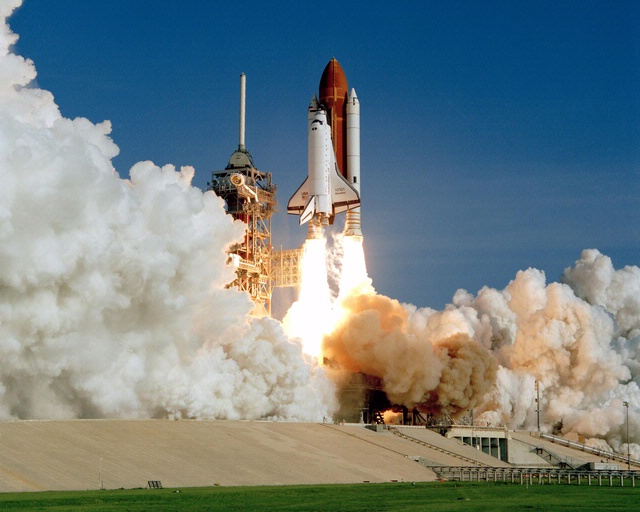
\includegraphics[scale=0.35]{gambar/roketluarangkasa.jpg}

  % Ubah dengan keterangan gambar yang diinginkan
  \caption{Peluncuran roket luar angkasa \emph{Discovery} \citep{roketluarangkasa}.}
  \label{fig:roketluarangkasa}
\end{figure}

Roket luar angkasa merupakan \lipsum[1]

\emph{Discovery}, Gambar \ref{fig:roketluarangkasa}, merupakan \lipsum[2]

% Per Teori Penunjang dibuat section baru

\section{Gravitasi}
\label{sec:gravitasi}

Gravitasi merupakan \lipsum[1]

\subsection{Hukum Newton}
\label{subsec:hukumnewton2}

Newton \citep{newton1687} pernah merumuskan bahwa \lipsum[1]
Kemudian menjadi persamaan seperti pada persamaan \ref{eq:hukumpertamanewton}.

% Contoh pembuatan persamaan
\begin{equation}
  \label{eq:hukumpertamanewton}
  \sum \mathbf{F} = 0\; \Leftrightarrow\; \frac{\mathrm{d} \mathbf{v} }{\mathrm{d}t} = 0.
\end{equation}

\subsection{Anti Gravitasi}
\label{subsec:antigravitasi}

Anti gravitasi merupakan \lipsum[1]

  \cleardoublepage

  % Bab 3 desain dan implementasi
  \chapter{METODOLOGI}
\label{chap:metodologi}

% Ubah bagian-bagian berikut dengan isi dari desain dan implementasi

Penelitian ini dilaksanakan sesuai \lipsum[1][1-5]


\section{Peralatan}
\label{sec:peralatan}

Alat yang digunakan yaitu: \lipsum[1]

\subsection{Perangkat}
\label{subsec:perangkat}

Perangkat yang digunakan menggunakan spesifikasi \lipsum[1]

\section{Desain Sistem}
\label{sec:desainsistem}

Sistem akan dibuat dengan \lipsum[1-2]

% Per blok diagram dijelaskan dan dibuatkan section masing-masing

% \section{Blok Diagram}
% \label{sec:blokdiagram}

% Contoh pembuatan potongan kode
\begin{lstlisting}[
  language=C++,
  caption={Program halo dunia.},
  label={lst:halodunia}
]
#include <iostream>

int main() {
    std::cout << "Halo Dunia!";
    return 0;
}
\end{lstlisting}

\lipsum[2-3]

% Contoh input potongan kode dari file
\lstinputlisting[
  language=Python,
  caption={Program perhitungan bilangan prima.},
  label={lst:bilanganprima}
]{program/bilangan-prima.py}

\lipsum[4]

  \cleardoublepage

  % Bab 4 pengujian dan analisis
  \chapter{HASIL DAN PEMBAHASAN}
\label{chap:hasilpembahasan}

% Ubah bagian-bagian berikut dengan isi dari hasil dan pembahasan

Pada penelitian ini dipaparkan \lipsum[1][1-5]

% Skenario pengujian berupa hasil penelitian dan perancangan yang telah dibuat pada bab 3

\section{Skenario Pengujian}
\label{sec:skenariopengujian}

Pengujian dilakukan dengan \lipsum[1-2]

\section{Evaluasi Pengujian}
\label{sec:analisispengujian}

Dari pengujian yang \lipsum[1]

% Contoh pembuatan tabel
\begin{longtable}{|c|c|c|}
  \caption{Hasil Pengukuran Energi dan Kecepatan}
  \label{tb:EnergiKecepatan}\\
  \hline
  \rowcolor[HTML]{C0C0C0}
  \textbf{Energi} & \textbf{Jarak Tempuh} & \textbf{Kecepatan} \\
  \hline
  10 J & 1000 M & 200 M/s \\
  20 J & 2000 M & 400 M/s \\
  30 J & 4000 M & 800 M/s \\
  40 J & 8000 M & 1600 M/s \\
  \hline
\end{longtable}

\lipsum[2-4]

  \cleardoublepage

  % Bab 5 penutup
  \chapter{PENUTUP}
\label{chap:penutup}

% Ubah bagian-bagian berikut dengan isi dari penutup

\section{Kesimpulan}
\label{sec:kesimpulan}

Berdasarkan hasil pengujian yang \lipsum[1][1-3] sebagai berikut:

\begin{enumerate}[nolistsep]

  \item Pembuatan \lipsum[2][1-3]

  \item \lipsum[2][4-6]

  \item \lipsum[2][7-10]

\end{enumerate}

\section{Saran}
\label{chap:saran}

Untuk pengembangan lebih lanjut pada \lipsum[1][1-3] antara lain:

\begin{enumerate}[nolistsep]

  \item Memperbaiki \lipsum[2][1-3]

  \item \lipsum[2][4-6]

  \item \lipsum[2][7-10]

\end{enumerate}

  \cleardoublepage

  % Daftar pustaka
  \renewcommand\bibname{DAFTAR PUSTAKA}
  \addcontentsline{toc}{chapter}{\bibname}
  \bibliographystyle{unsrtnat}
  \bibliography{pustaka/pustaka.bib}
  \cleardoublepage

  % Biografi penulis
  \begin{center}
  \Large
  \textbf{BIOGRAFI PENULIS}
\end{center}

\addcontentsline{toc}{chapter}{BIOGRAFI PENULIS}

\vspace{2ex}

\begin{wrapfigure}{L}{0.3\textwidth}
  \centering
  \vspace{-3ex}
  % Ubah file gambar berikut dengan file foto dari mahasiswa
  
\includegraphics[width=0.3\textwidth]{gambar/elon.jpg}
  \vspace{-4ex}
\end{wrapfigure}

% Ubah kalimat berikut dengan biografi dari mahasiswa
Elon Reeve Musk, lahir pada \lipsum[1]

\lipsum[2]

  \cleardoublepage

\end{document}
